\documentclass[10pt,a4paper]{article}
\usepackage{ucs}
\usepackage[utf8x]{inputenc}
\usepackage{amsmath}
\usepackage{amsfonts}
\usepackage{amssymb}
\usepackage[pdftex]{graphicx}

\usepackage[slovene]{babel}
\usepackage{lmodern}
\usepackage[T1]{fontenc}

\author{Vida Groznik, Anže Starič}
\title{Spomin}

\begin{document}
\maketitle
\newpage

\section{Uvod}
Spomin igra pomembno vlogo v našem življenju, saj predstavlja osnovo za učenje, sklepanje in razumevanje. Brez spomina bi dojemali le sedanjost in nebi mogli razumeti vzročnosti, saj bi do trenutka, ko bi videli rezultat neke akcije že pozabili, da smo akcijo izvedli.

Spomin v grobem delimo na eksplicitni (deklarativni) in implicitni (nedeklarativni) spomin. Kadar govorimo preprosto o spominu najpogosteje mislimo na {\bf eksplicitni spomin}. Do eksplicitnih spominov lahko dostopamo zavestno, enostavno jih tvorimo, ravno tako enostavno jih pozabljamo.

{\bf Implicitnega spomina} po drugi strani ne moremo uporabljati zavestno, vendar naučena opravila lahko opravljamo tudi brez zavestnega priklica (vožnja kolesa, prostoročno tipkanje, ...). Za tvorjenje implicitnih spominov potrebujemo več ponavljanja in vaje kot za tvorjenje eksplicitnih spominov, vendar jih zato težje pozabimo.

\section{Eksplicitni spomin}
Kot smo omenili v uvodu, eksplicitne spomine tvorimo in do njih dostopamo zavestno. Spominsko delovanje ločimo na pet procesov: {\it pozornost}, {\it vkodiranje}, {\it shranjevanje}, {\it konsolidacija} in {\it obnavljanje informacij}. {\it Pozornost} je sposobnost osredotočanja na določeno nalogo in igra pomembno vlogo pri izboru informacij, ki vstopajo v spominski proces. Drugi korak je {\it vkodiranje}, ki predstavlja registracijo informacij med procesom učenja. Če lahko informacijo povežemo z že znanimi asociacijami, je postopek vkodiranja bolj učinkovit. Ko je informacija vkodirana je {\it shranjena} v kratkoročni spomin. {\it Konsolidacija} je postopek organizacije kompleksnih informacij, pri katerem se prenesejo v dolgoročni spomin. Pri dostopanju do informacij gre za procese {\it obnavljanja informacij}, poznamo spontan priklic, priklic s pomočjo namiga in prepoznavanje. S priklicom in prepoznavanjem najlažje merimo sposobnost posameznikovega spominskega sistema.

Postopno pozabljanje je običajen proces našega spominskega sistema, kadar pa pride do večje izgube spomina, ki je posledica bolezni ali poškodbe govorimo o amneziji. Poznamo dve vrsti amnezije, {\it retrogradno amnezijo}, pri kateri gre za izgubo spominov pred poškodbo in {\it anterogradno amnezijo}, pri kateri gre za nezmožnost tvorjenja spominov po poškodbi. Bolnik, ki je doživel poškodbo pri 32 letih, katere posledica je bila retrogradna amnezija se tako ne more spomniti dgodkov, ki so se zgodili med njegovim 30 in 32 letom, če pa je posledica anterogradna amnezija, se ne more spomniti ničesar, kar se je zgodilo po njegovem 32 letu.

\subsection{Temporalni reženj}
\begin{figure}[h]
  \centering
    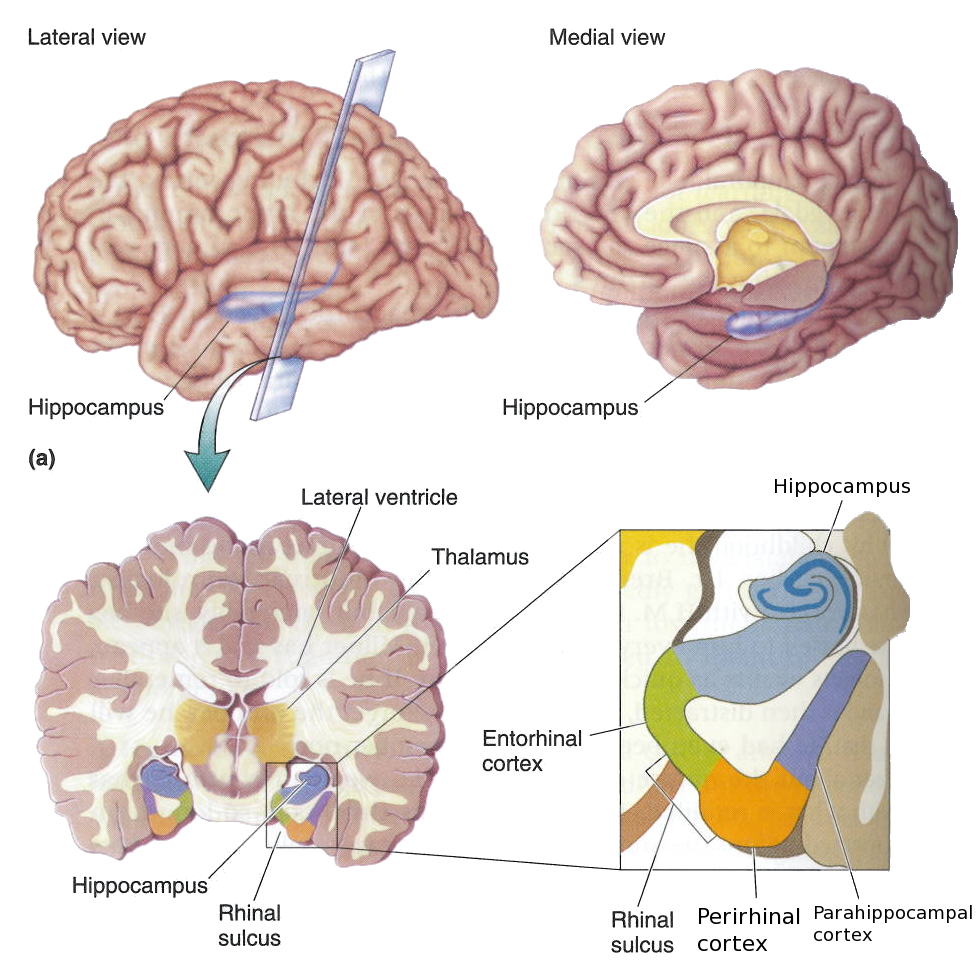
\includegraphics[width=1.0\textwidth]{LokacijaHippocampusa.png}
  \caption{Kje se nahaja hippocampus}
  \label{sHippocampus}
\end{figure}

\subsubsection{Bolnik H.M.}
Pri bolniku H.M so se okrog desetega leta začeli pojavljati epileptični napadi. Z leti so postajali vse hujši, vključevali so tresenje, grizenje jezika in izgubo zavesti. Ker zaradi epilepsije kljub jemanju zdravil ni mogel normalno delati, so mu pri 27 letih med operacijo izrezali dela obeh temporalnih režnjev. Od operacije dalje se pri bolniku epileptični napadi niso več pojavljali.

Odstranitev temporalnih režnjev ni vplivala na zavedanje, inteligenco ali osebnost bolnika H.M., vendar se je pri njem pojavila huda oblika amnezije. Opazni so bili znaki obeh vrst amnezije. Delna retrogradna amnezija se je kazala kot izguba spomina o dogodkih nekaj let pred operacijo, vendar je bolnik še vedno lahko priklical določene spomine iz otroštva. Anterogradna amnezija je bila prisotna v hujši obliki, zaradi nje bolnik ni prepoznal stvari, ki jih je spoznal nekaj minut nazaj. Bolnik si ni zapomnil niti zdravnice, ki je z njim delala vsak dan skoraj 50 let. Pri izvajanju preizkusa delovnega spomina (pomnjenje zaporedja števil) je bolnik dosegel običajen rezultat. V primeru, da je med izvajanjem poizkusa preusmeril pozornost na nekaj drugega, pa je poleg števil pozabil tudi, da si je moral zapomniti števila.

\subsubsection{Vloga temporalnega režnja}
Iz primera bolnika H. M. lahko sklepamo, da po odstranitvi medialnih temporalnih režnjev dolgoročni in delovni spomin nista bila poškodovana, pojavila pa se je okvara sistemov za tvorjenje novih spominov. Pri operaciji so bili odstranjeni del hippocampusa, amygdala ter del korteksa (rhinalni sulcus in parahipocampalni cortex). Če opazujemo povezave v možganih opazimo, da vhod v medialni temporalni reženj prihaja iz asociacijskih področij. Informacije prehajajo preko korteksa do hippocampusa. V asociacijskih področjih se nahajajo močno obdelane informacije različnih modalnosti, kar pomeni, da vhod predstavljajo kompleksne predstavitve. Glavna izhodna povezava je {\it fornix}, ki gre mimo thalamusa in se konča v hypothalamusu.

Hippocampus skupaj z bližnjim korteksom sodeluje pri pretvarjanju informacij, ki prihajajo iz asociacijskih področij. Izgleda tudi, da strukture medialnih temporalnih režnjev sodelujejo pri konsolidaciji spominov. Hkraten pojav retrogradne in anterogradne amnezije pri bolnikih z okvaro medialnih temporalnih struktur namiguje tudi, da se v tem področju nekaj časa hranijo spomini, dokler se dokončno ne konsolidirajo v neokorteksu.

\section{Diencephalon}
\subsection{Bolnik N.A.}
N.A. je bil po poklicu vzdrževalec radarjev v ameriških zračnih silah. Nekega dne je sestavljal model letala, njegov cimer pa je za njegovim hrbtom vadil mečevanje. Ko se je N.A. v nepravem trenutku obrnil, se mu je meč skozi desno nosnico zapičil v možgane. Čez več let so ugotovili, da mu je pri te meč poškodoval le levi del thalamusa, ostali del možganov je bil nepoškodovan.

Po okrevanju se je kognitivna sposobnost vrnila na normalen nivo, vendar pa je imel težave s spominom. Imel je retrogradno amnezijo za obdobje dveh let pred nesrečo in precej hudo obliko anterogradne amnezije. Le-ta ni bila tako huda kot pri bolniku H.M, saj se je lahko spomnil nekaterih dogodkov in obrazov po nesreči, vendar so bili spomini površni. Čeprav je bila amnezija bolnika N.A. blažja, je po znakih zelo podobna amneziji bolnika H.M, delovni in dolgoročni spomin nista bila prizadeta, imel pa je težave s tvorjenjem novih spominov in retrogradno amnezijo, iz česar sklepamo, da tudi thalamus igra pomembno vlogo pri konsolidaciji spominov.



\section{Implicitni spomin}
\subsection{Proceduralni spomin}
Za proceduralni spomin bi v grobem lahko rekli, da je to spomin za opravljanje različnih nalog. Ko se pojavi potreba po opravljanju neke naloge, se avtomatsko prikliče in uporabi proceduralni spomin, ki vsebuje tako kognitivne kot tudi motorične spretnosti. Proceduralni spomin je vrsta dolgoročnega spomina, natančneje implicitnega spomina.

\subsubsection{Anatomska struktura}
Striatum in bazalni gangliji\\
cerebellum\\
limbični sistem

\subsubsection{Fiziologija}
Dopamin\\
sinapsa

\subsubsection{Testi}

\subsubsection{Motnje}
Alzheimerjeva bolezen in demenca\\
Sindrom Gilles de la tourete\\
Virus HIV\\
Huntingtonova bolezen\\
Obsesivna kompulzivna motnja (OCD)\\
Parkinsonova bolezen\\
Šizofrenija

\subsubsection{Vpliv drog}
Alkohol\\
Kokain\\
Psihostimulanti

\section{}
\end{document}